% Options for packages loaded elsewhere
\PassOptionsToPackage{unicode}{hyperref}
\PassOptionsToPackage{hyphens}{url}
\PassOptionsToPackage{dvipsnames,svgnames,x11names}{xcolor}
%
\documentclass[
]{article}
\usepackage{amsmath,amssymb}
\usepackage{iftex}
\ifPDFTeX
  \usepackage[T1]{fontenc}
  \usepackage[utf8]{inputenc}
  \usepackage{textcomp} % provide euro and other symbols
\else % if luatex or xetex
  \usepackage{unicode-math} % this also loads fontspec
  \defaultfontfeatures{Scale=MatchLowercase}
  \defaultfontfeatures[\rmfamily]{Ligatures=TeX,Scale=1}
\fi
\usepackage{lmodern}
\ifPDFTeX\else
  % xetex/luatex font selection
\fi
% Use upquote if available, for straight quotes in verbatim environments
\IfFileExists{upquote.sty}{\usepackage{upquote}}{}
\IfFileExists{microtype.sty}{% use microtype if available
  \usepackage[]{microtype}
  \UseMicrotypeSet[protrusion]{basicmath} % disable protrusion for tt fonts
}{}
\makeatletter
\@ifundefined{KOMAClassName}{% if non-KOMA class
  \IfFileExists{parskip.sty}{%
    \usepackage{parskip}
  }{% else
    \setlength{\parindent}{0pt}
    \setlength{\parskip}{6pt plus 2pt minus 1pt}}
}{% if KOMA class
  \KOMAoptions{parskip=half}}
\makeatother
\usepackage{xcolor}
\usepackage[margin=1in]{geometry}
\usepackage{color}
\usepackage{fancyvrb}
\newcommand{\VerbBar}{|}
\newcommand{\VERB}{\Verb[commandchars=\\\{\}]}
\DefineVerbatimEnvironment{Highlighting}{Verbatim}{commandchars=\\\{\}}
% Add ',fontsize=\small' for more characters per line
\usepackage{framed}
\definecolor{shadecolor}{RGB}{248,248,248}
\newenvironment{Shaded}{\begin{snugshade}}{\end{snugshade}}
\newcommand{\AlertTok}[1]{\textcolor[rgb]{0.94,0.16,0.16}{#1}}
\newcommand{\AnnotationTok}[1]{\textcolor[rgb]{0.56,0.35,0.01}{\textbf{\textit{#1}}}}
\newcommand{\AttributeTok}[1]{\textcolor[rgb]{0.13,0.29,0.53}{#1}}
\newcommand{\BaseNTok}[1]{\textcolor[rgb]{0.00,0.00,0.81}{#1}}
\newcommand{\BuiltInTok}[1]{#1}
\newcommand{\CharTok}[1]{\textcolor[rgb]{0.31,0.60,0.02}{#1}}
\newcommand{\CommentTok}[1]{\textcolor[rgb]{0.56,0.35,0.01}{\textit{#1}}}
\newcommand{\CommentVarTok}[1]{\textcolor[rgb]{0.56,0.35,0.01}{\textbf{\textit{#1}}}}
\newcommand{\ConstantTok}[1]{\textcolor[rgb]{0.56,0.35,0.01}{#1}}
\newcommand{\ControlFlowTok}[1]{\textcolor[rgb]{0.13,0.29,0.53}{\textbf{#1}}}
\newcommand{\DataTypeTok}[1]{\textcolor[rgb]{0.13,0.29,0.53}{#1}}
\newcommand{\DecValTok}[1]{\textcolor[rgb]{0.00,0.00,0.81}{#1}}
\newcommand{\DocumentationTok}[1]{\textcolor[rgb]{0.56,0.35,0.01}{\textbf{\textit{#1}}}}
\newcommand{\ErrorTok}[1]{\textcolor[rgb]{0.64,0.00,0.00}{\textbf{#1}}}
\newcommand{\ExtensionTok}[1]{#1}
\newcommand{\FloatTok}[1]{\textcolor[rgb]{0.00,0.00,0.81}{#1}}
\newcommand{\FunctionTok}[1]{\textcolor[rgb]{0.13,0.29,0.53}{\textbf{#1}}}
\newcommand{\ImportTok}[1]{#1}
\newcommand{\InformationTok}[1]{\textcolor[rgb]{0.56,0.35,0.01}{\textbf{\textit{#1}}}}
\newcommand{\KeywordTok}[1]{\textcolor[rgb]{0.13,0.29,0.53}{\textbf{#1}}}
\newcommand{\NormalTok}[1]{#1}
\newcommand{\OperatorTok}[1]{\textcolor[rgb]{0.81,0.36,0.00}{\textbf{#1}}}
\newcommand{\OtherTok}[1]{\textcolor[rgb]{0.56,0.35,0.01}{#1}}
\newcommand{\PreprocessorTok}[1]{\textcolor[rgb]{0.56,0.35,0.01}{\textit{#1}}}
\newcommand{\RegionMarkerTok}[1]{#1}
\newcommand{\SpecialCharTok}[1]{\textcolor[rgb]{0.81,0.36,0.00}{\textbf{#1}}}
\newcommand{\SpecialStringTok}[1]{\textcolor[rgb]{0.31,0.60,0.02}{#1}}
\newcommand{\StringTok}[1]{\textcolor[rgb]{0.31,0.60,0.02}{#1}}
\newcommand{\VariableTok}[1]{\textcolor[rgb]{0.00,0.00,0.00}{#1}}
\newcommand{\VerbatimStringTok}[1]{\textcolor[rgb]{0.31,0.60,0.02}{#1}}
\newcommand{\WarningTok}[1]{\textcolor[rgb]{0.56,0.35,0.01}{\textbf{\textit{#1}}}}
\usepackage{longtable,booktabs,array}
\usepackage{calc} % for calculating minipage widths
% Correct order of tables after \paragraph or \subparagraph
\usepackage{etoolbox}
\makeatletter
\patchcmd\longtable{\par}{\if@noskipsec\mbox{}\fi\par}{}{}
\makeatother
% Allow footnotes in longtable head/foot
\IfFileExists{footnotehyper.sty}{\usepackage{footnotehyper}}{\usepackage{footnote}}
\makesavenoteenv{longtable}
\usepackage{graphicx}
\makeatletter
\def\maxwidth{\ifdim\Gin@nat@width>\linewidth\linewidth\else\Gin@nat@width\fi}
\def\maxheight{\ifdim\Gin@nat@height>\textheight\textheight\else\Gin@nat@height\fi}
\makeatother
% Scale images if necessary, so that they will not overflow the page
% margins by default, and it is still possible to overwrite the defaults
% using explicit options in \includegraphics[width, height, ...]{}
\setkeys{Gin}{width=\maxwidth,height=\maxheight,keepaspectratio}
% Set default figure placement to htbp
\makeatletter
\def\fps@figure{htbp}
\makeatother
\setlength{\emergencystretch}{3em} % prevent overfull lines
\providecommand{\tightlist}{%
  \setlength{\itemsep}{0pt}\setlength{\parskip}{0pt}}
\setcounter{secnumdepth}{-\maxdimen} % remove section numbering
\newlength{\cslhangindent}
\setlength{\cslhangindent}{1.5em}
\newlength{\csllabelwidth}
\setlength{\csllabelwidth}{3em}
\newlength{\cslentryspacingunit} % times entry-spacing
\setlength{\cslentryspacingunit}{\parskip}
\newenvironment{CSLReferences}[2] % #1 hanging-ident, #2 entry spacing
 {% don't indent paragraphs
  \setlength{\parindent}{0pt}
  % turn on hanging indent if param 1 is 1
  \ifodd #1
  \let\oldpar\par
  \def\par{\hangindent=\cslhangindent\oldpar}
  \fi
  % set entry spacing
  \setlength{\parskip}{#2\cslentryspacingunit}
 }%
 {}
\usepackage{calc}
\newcommand{\CSLBlock}[1]{#1\hfill\break}
\newcommand{\CSLLeftMargin}[1]{\parbox[t]{\csllabelwidth}{#1}}
\newcommand{\CSLRightInline}[1]{\parbox[t]{\linewidth - \csllabelwidth}{#1}\break}
\newcommand{\CSLIndent}[1]{\hspace{\cslhangindent}#1}
\usepackage{fancyhdr}
\pagestyle{fancy}
\fancyhf{}
\lfoot[\thepage]{}
\rfoot[]{\thepage}
\fontsize{12}{22}
\selectfont
\usepackage{booktabs}
\usepackage{longtable}
\usepackage{array}
\usepackage{multirow}
\usepackage{wrapfig}
\usepackage{float}
\usepackage{colortbl}
\usepackage{pdflscape}
\usepackage{tabu}
\usepackage{threeparttable}
\usepackage{threeparttablex}
\usepackage[normalem]{ulem}
\usepackage{makecell}
\usepackage{xcolor}
\ifLuaTeX
  \usepackage{selnolig}  % disable illegal ligatures
\fi
\IfFileExists{bookmark.sty}{\usepackage{bookmark}}{\usepackage{hyperref}}
\IfFileExists{xurl.sty}{\usepackage{xurl}}{} % add URL line breaks if available
\urlstyle{same}
\hypersetup{
  colorlinks=true,
  linkcolor={blue},
  filecolor={Maroon},
  citecolor={Blue},
  urlcolor={Blue},
  pdfcreator={LaTeX via pandoc}}

\title{
\includegraphics[width=10cm,height=\textheight]{IEO-logo2.png}}
\author{}
\date{\vspace{-2.5em}}

\begin{document}
\maketitle


\pagenumbering{gobble}

%\begin{titlepage}
\begin{flushleft}
\Large{\textbf{Working Paper}}\\
\vspace*{2\baselineskip}
\LARGE{\textbf{Methodological implementation of Swept Area Ratio (SAR) in the wedge clam fishery \textit{Chamelea galllina} in the Gulf of Cádiz, Spain}}\\
\vspace*{5\baselineskip}
\Large{FEMP 04 Project}\\
\vspace*{1\baselineskip}
\Large{Instituto Español de Oceanografía, Cádiz }\\
\vspace*{4\baselineskip}
\end{flushleft}
\begin{flushright}
\large{\textit{Magro, Ana}}\\
\large{\textit{Mardones, Mauricio}}\\
\large{\textit{Delgado, Marina}}\\
\vspace*{1\baselineskip}
\normalsize{\textbf{Date}}\\
Abril, 2024
\end{flushright}

% \end{titlepage}


\hypersetup{linkcolor = black}
\newpage
\pagenumbering{roman}
%\tableofcontents
%\addcontentsline{toc}{section}{\contentsname}

\newpage



\pagenumbering{arabic}
\hypersetup{linkcolor = blue}

{
\hypersetup{linkcolor=}
\setcounter{tocdepth}{3}
\tableofcontents
}
\newpage

\hypertarget{introduction}{%
\section{INTRODUCTION}\label{introduction}}

\hypertarget{methodology}{%
\section{METHODOLOGY}\label{methodology}}

\hypertarget{data-satelital-vessel}{%
\subsection{DATA SATELITAL VESSEL}\label{data-satelital-vessel}}

Por ahora solo trabajaremos con la data entregada por Candelaria Burgos para Chirla, que son los datos del año 2008 y 2009.

\begin{verbatim}
## [1] 1554983      21
\end{verbatim}

\hypertarget{results}{%
\subsection{RESULTS}\label{results}}

Identifico la cantidad de embarcaciones presentes en la BD

\begin{Shaded}
\begin{Highlighting}[]
\FunctionTok{unique}\NormalTok{(cajas2009uni}\SpecialCharTok{$}\NormalTok{MATRICULA)}
\end{Highlighting}
\end{Shaded}

\begin{verbatim}
##  [1] "SE-1-768"   "HU-2-2158"  "HU-2-1931"  "SE-1-792"   "HU-3-1512" 
##  [6] "HU-2-2207"  "HU-3-5-91"  "AL-2-1833"  "HU-2-1-95"  "SE-1-1-95" 
## [11] "HU-2-3-95"  "HU-2-2-95"  "HU-1-5-96"  "HU-2-7-97"  "HU-2-1-97" 
## [16] "HU-2-5-96"  "HU-2-3-96"  "HU-2-3-98"  "HU-3-11-98" "HU-2-4-98" 
## [21] "HU-2-3-97"  "SE-1-4-98"  "HU-3-3-99"  "HU-2-8-98"  "HU-3-2-99" 
## [26] "HU-2-3-99"  "HU-2-8-99"  "HU-2-9-99"  "HU-2-13-99" "HU-2-14-99"
## [31] "HU-2-8-00"  "HU-3-8-00"  "HU-3-10-00" "HU-3-1-01"  "HU-2-5-01" 
## [36] "HU-2-9-01"  "HU-3-4-01"  "HU-3-13-00" "HU-2-17-01" "SE-1-8-01" 
## [41] "HU-2-7-01"  "HU-3-1-02"  "HU-2-28-01" "HU-2-7-02"  "HU-2-8-02" 
## [46] "HU-2-16-02" "HU-2-17-02" "HU-3-9-02"  "HU-3-14-02" "HU-3-6-02" 
## [51] "HU-3-4-02"  "SE-1-10-03" "HU-3-12-02" "HU-2-14-03" "HU-3-11-02"
## [56] "HU-2-27-03" "HU-2-29-03" "HU-2-5-04"  "HU-3-1-04"  "HU-2-9-04" 
## [61] "HU-1-3-04"  "HU-3-8-04"  "HU-1-4-05"  "HU-2-13-05" "HU-3-2-04" 
## [66] "HU-3-7-05"  "HU-3-2-05"  "HU-3-4-05"  "HU-3-9-05"  "HU-3-8-05" 
## [71] "HU-3-6-04"  "HU-3-1-06"  "HU-2-4-06"  "HU-3-5-05"  "HU-3-5-06" 
## [76] "HU-2-2-07"  "HU-3-1164"  "HU-2-8-97"  "HU-2-11-99" "HU-2-19-01"
## [81] "SE-1-14-04" "HU-2-1-06"  "HU-2-2-06"  "SE-1-15-03" "HU-3-5-02" 
## [86] "HU-2-15-01" "HU-2-13-02" "HU-3-16-02" "HU-2-1218"  "HU-2-12-02"
## [91] "SE-1-14-03" "HU-3-10-04" "HU-2-8-01"
\end{verbatim}

De forma simple compruenbo los meses y dias con actividad de los datos sin filtrar;

Los métodos para la estimación y cartografiado del esfuerzo pesquero a partir de los datos de los VMS ya se han estudiado en varias pesquerías anteriormente. Estos estudios recomiendan un proceso en varios pasos según (\protect\hyperlink{ref-Cojan2012}{\textbf{Cojan2012?}}):

1- Borrar los registros duplicados,

2- Borrar los registros en puertos.

\begin{center}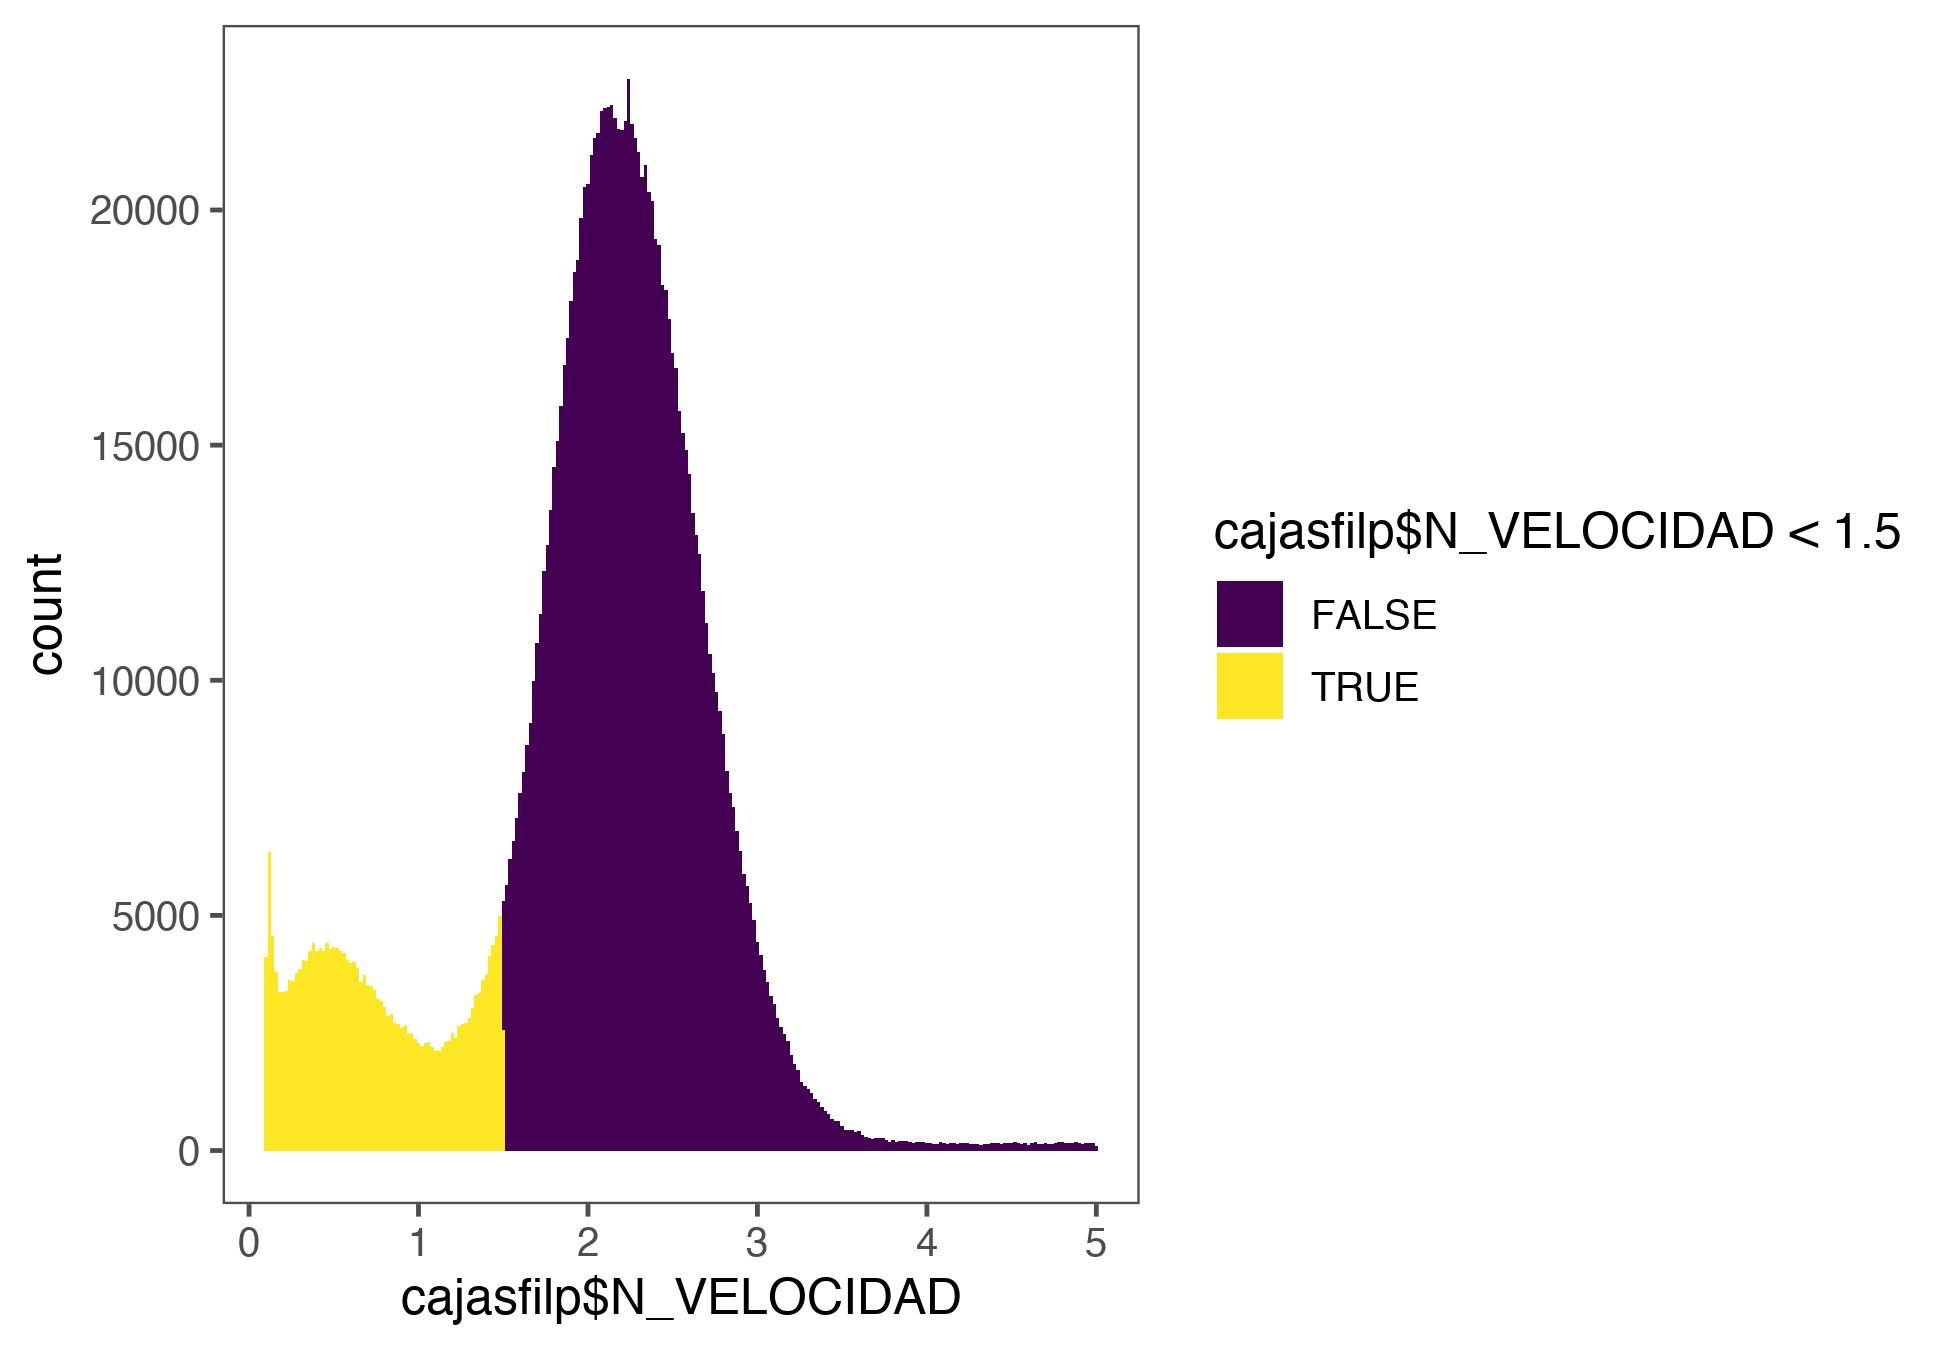
\includegraphics{SAR_Method_files/figure-latex/unnamed-chunk-8-1} \end{center}

3- Calcular el intervalo de tiempo entre registros sucesivos,

La idea es identificar los registros con tiempo efectivo de arrastre como lo muestra la Figura \ref{fig:esq};

\begin{figure}

{\centering \includegraphics[width=0.5\linewidth]{FIG/umbralveloc} 

}

\caption{\label{esq}Umbrarl de definiciones para calculo de velocidad de arrantre}\label{fig:esq}
\end{figure}

De esta forma, a cada señal proporcionada por la caja verde se le asignó una actividad: pesca, maniobra o navegada. En la figura 8 se puede ver un histograma que representa el número de registros en función de la velocidad para los registros filtrados, en él se observa cómo han desaparecido los registros en puerto y que existen tres modas correspondientes a las actividades mencionadas, maniobras (M), pesca (P) y navegaciones (N). (\protect\hyperlink{ref-Cohan2012}{Cojan, 2012})

Los registros en los cuales la velocidad del buque fue inferior a 1.5 nudos o entre 3.5 y 6 nudos, fueron considerados como maniobras de pesca (actividad ``M''), tales como la virada y largada del arte o el reposicionamiento del buque precedente al arrastre.

\begin{verbatim}
##                     FK_ERES      FECHA DIA     HORA FK_BUQUE MATRICULA   PUERTO
## Draga_01_2009.txt.1     601 2009-01-29  29 13:31:17     9883  SE-1-768 SANLUCAR
## Draga_01_2009.txt.2     601 2009-01-29  29 13:39:15     9883  SE-1-768 SANLUCAR
## Draga_01_2009.txt.3     601 2009-01-29  29 13:42:13     9883  SE-1-768 SANLUCAR
## Draga_01_2009.txt.4     601 2009-01-29  29 13:51:13     9883  SE-1-768 SANLUCAR
## Draga_01_2009.txt.5     601 2009-01-30  30 11:01:20     9883  SE-1-768 SANLUCAR
## Draga_01_2009.txt.6     601 2009-01-30  30 12:22:22     9883  SE-1-768 SANLUCAR
##                     FK_TIPO_F F_LOCALIZA N_LONGITUD N_LATITUD      N_X     N_Y
## Draga_01_2009.txt.1         3  29-JAN-09  -6.338148  36.80516 202279.3 4078662
## Draga_01_2009.txt.2         3  29-JAN-09  -6.338153  36.80516 202278.8 4078661
## Draga_01_2009.txt.3         3  29-JAN-09  -6.338127  36.80516 202281.2 4078662
## Draga_01_2009.txt.4         3  29-JAN-09  -6.338148  36.80515 202279.2 4078661
## Draga_01_2009.txt.5         3  30-JAN-09  -6.451208  36.87560 192471.5 4086838
## Draga_01_2009.txt.6         3  30-JAN-09  -6.360342  36.79270 200249.9 4077348
##                     N_VELOCIDAD N_RUMBO N_SATELITES N_EN_PUERTO L_BACKUP
## Draga_01_2009.txt.1     0.10799  22.100           5           0        0
## Draga_01_2009.txt.2     0.11879  66.224           7           1        0
## Draga_01_2009.txt.3     0.14039  87.848           8           1        0
## Draga_01_2009.txt.4     0.10799 114.800           8           1        0
## Draga_01_2009.txt.5     1.83423  12.982           9           0        0
## Draga_01_2009.txt.6     0.76350 260.670           7           0        0
##                     FK_ACTIVI FK_ESTADO FK_MODAL  ANO MES
## Draga_01_2009.txt.1         3         5        0 2009   1
## Draga_01_2009.txt.2         1         5        0 2009   1
## Draga_01_2009.txt.3         1         5        0 2009   1
## Draga_01_2009.txt.4         1         5        0 2009   1
## Draga_01_2009.txt.5         4         3        3 2009   1
## Draga_01_2009.txt.6         3         3        0 2009   1
\end{verbatim}

\begin{verbatim}
## [1] 1468527      24
\end{verbatim}

4- Ahora calculo las distancias entre puntos. como??

\hypertarget{muxe9todo-1}{%
\subsubsection{Método 1}\label{muxe9todo-1}}

\begin{verbatim}
##                        FK_ERES      FECHA DIA     HORA FK_BUQUE  MATRICULA
## Draga_05_2008.txt.184      631 2008-05-01   1 00:51:06    23032  SE-1-1-95
## Draga_05_2008.txt.186      631 2008-05-01   1 01:11:06    23032  SE-1-1-95
## Draga_05_2008.txt.3676     541 2008-05-01   1 02:37:55    25545 SE-1-10-03
## Draga_05_2008.txt.276      607 2008-05-01   1 03:23:14    23266  HU-2-3-95
## Draga_05_2008.txt.3374     542 2008-05-01   1 03:28:42    25111  SE-1-8-01
## Draga_05_2008.txt.188      631 2008-05-01   1 03:31:06    23032  SE-1-1-95
##                               PUERTO FK_TIPO_F F_LOCALIZA N_LONGITUD N_LATITUD
## Draga_05_2008.txt.184       SANLUCAR         3  01-MAY-08  -6.338002  36.80437
## Draga_05_2008.txt.186       SANLUCAR         3  01-MAY-08  -6.338000  36.80437
## Draga_05_2008.txt.3676      SANLUCAR         3  01-MAY-08  -6.338063  36.80459
## Draga_05_2008.txt.276  ISLA CRISTINA         3  01-MAY-08  -6.962827  37.18792
## Draga_05_2008.txt.3374      SANLUCAR         3  01-MAY-08  -6.337983  36.80457
## Draga_05_2008.txt.188       SANLUCAR         3  01-MAY-08  -6.338008  36.80435
##                             N_X     N_Y N_VELOCIDAD N_RUMBO N_SATELITES
## Draga_05_2008.txt.184  202289.3 4078573     0.11825 167.170           9
## Draga_05_2008.txt.186  202289.4 4078573     0.11825 159.820           9
## Draga_05_2008.txt.3676 202284.6 4078598     0.11285  48.787           8
## Draga_05_2008.txt.276  148294.7 4123282     0.11393  56.740           7
## Draga_05_2008.txt.3374 202291.7 4078596     0.12959 145.320           8
## Draga_05_2008.txt.188  202288.6 4078571     0.21544 154.960           8
##                        N_EN_PUERTO L_BACKUP FK_ACTIVI FK_ESTADO FK_MODAL  ANO
## Draga_05_2008.txt.184            1        0         1         5        0 2008
## Draga_05_2008.txt.186            1        0         1         5        0 2008
## Draga_05_2008.txt.3676           1        0         1         5        0 2008
## Draga_05_2008.txt.276            1        0         2         5        0 2008
## Draga_05_2008.txt.3374           1        0         1         5        0 2008
## Draga_05_2008.txt.188            1        0         1         5        0 2008
##                        MES MANIOBRA          fecha_hora    DISTANCIA
## Draga_05_2008.txt.184    5        M 2008-05-01 00:51:06           NA
## Draga_05_2008.txt.186    5        M 2008-05-01 01:11:06 2.378859e-01
## Draga_05_2008.txt.3676   5        M 2008-05-01 02:37:55 2.510427e+01
## Draga_05_2008.txt.276    5        M 2008-05-01 03:23:14 6.996624e+04
## Draga_05_2008.txt.3374   5        M 2008-05-01 03:28:42 6.997312e+04
## Draga_05_2008.txt.188    5        M 2008-05-01 03:31:06 2.456393e+01
\end{verbatim}

\hypertarget{muxe9todo-2}{%
\subsubsection{Método 2}\label{muxe9todo-2}}

Probar forma que indica Ana Magro, que es calcular tiempo de arrastre X Velocidad. La idea es calcular el tiempo entre registros dado por \texttt{fecha\_hora}. Y multiplicamos por \texttt{N\_VELOCIDAD}

5- Diferenciar entre registros de pesca y no pesca basándose en la velocidad y solo dejó los registros \texttt{P}

ahora dejo valores de distancia menores a 1 km (preguntar). Luego calculo las variables de velocidad en metros/seg. y tiempo recorrido por la rastra.

Gafico velocidad y SA promedio por barco

\begin{center}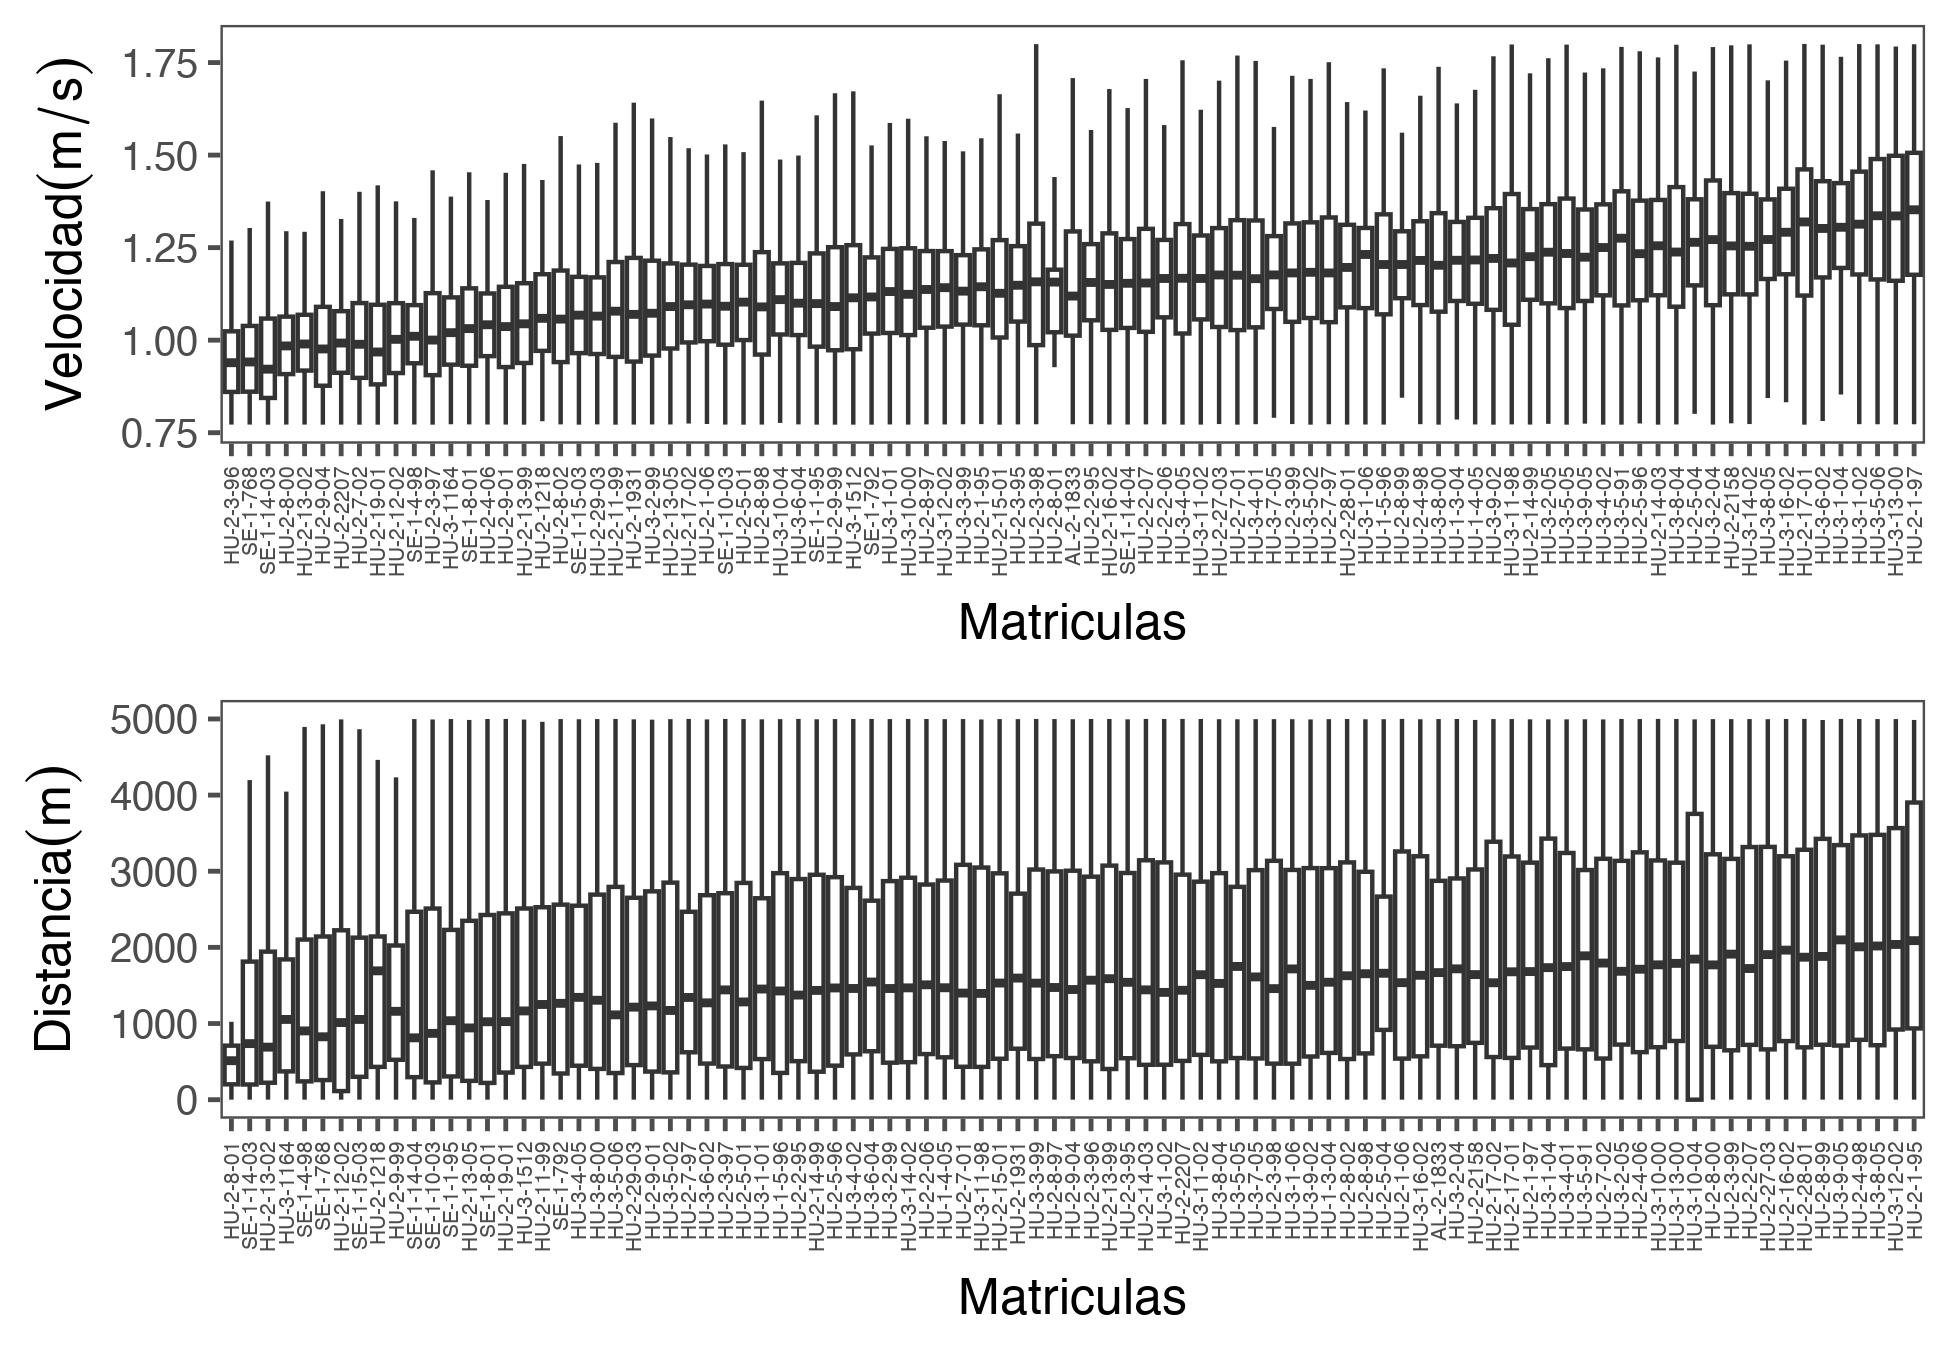
\includegraphics{SAR_Method_files/figure-latex/unnamed-chunk-14-1} \end{center}

Calculo el SAR

De acuerdo a Church et al. (\protect\hyperlink{ref-Church2016}{2016}), el cálculo de la Razón del Área Barrida (Swept Area Ratio, SAR) \texttt{SA} es el área barrida (mts/2), \texttt{CA} es el área de la celda y \texttt{SAR} es la proporción del área barrida (equivalente al número de veces que la celda fue barrida).

donde;

\[
SAr = \frac{SA}{CA}
\]

donde \texttt{SA}sera la distancia recorrida el arrastre y la apertura en metros del draga, es decir;

\[
SA = Distancia \times Apertura \ Draga
\]
Pero primero, debemos engrillar la data y luego calcular por cada celda

Ahora produzco un mapa de las grillas utilizadas en la pesquería de Chirla. Estos datos vectoriales fueron obtenidos desde la paina oficial de datos espaciales de la Junta de Andalucia \href{https://portalrediam.cica.es/descargas?path=\%2F08_AMBITOS_INTERES_AMBIENTAL\%2F02_LITORAL_MARINO\%2F04_SOCIOECONOMIA\%2FZonasProduccionMoluscos}{Shapesfile}

\hypertarget{leo-shapes-y-transformo-a-la-proyecciuxf3n-correcta.}{%
\subsection{Leo Shapes y transformo a la proyección correcta.}\label{leo-shapes-y-transformo-a-la-proyecciuxf3n-correcta.}}

\begin{verbatim}
## Reading layer `costa_proyectada' from data source 
##   `/Users/mauriciomardones/IEO/IN_BENTOS/SHP_Chirla/costa_proyectada.shp' 
##   using driver `ESRI Shapefile'
## Simple feature collection with 10 features and 4 fields
## Geometry type: POLYGON
## Dimension:     XY
## Bounding box:  xmin: -34115.27 ymin: 3891271 xmax: 301588.8 ymax: 4173659
## Projected CRS: WGS_1984_Complex_UTM_Zone_30N
\end{verbatim}

\begin{verbatim}
## Reading layer `cuadriculas_definitivo' from data source 
##   `/Users/mauriciomardones/IEO/IN_BENTOS/SHP_Chirla/cuadriculas_definitivo.shp' 
##   using driver `ESRI Shapefile'
## Simple feature collection with 219 features and 2 fields
## Geometry type: POLYGON
## Dimension:     XY
## Bounding box:  xmin: 109273.6 ymin: 4071852 xmax: 198073.5 ymax: 4125446
## Projected CRS: ETRS89 / UTM zone 30N
\end{verbatim}

\begin{verbatim}
## Reading layer `batimetria_rediam20x20_10m_id' from data source 
##   `/Users/mauriciomardones/IEO/IN_BENTOS/SHP_Chirla/batimetria_rediam20x20_10m_id.shp' 
##   using driver `ESRI Shapefile'
## Simple feature collection with 1 feature and 1 field
## Geometry type: MULTIPOLYGON
## Dimension:     XY
## Bounding box:  xmin: 99337.29 ymin: 4070000 xmax: 201873.6 ymax: 4127412
## Projected CRS: ETRS89 / UTM zone 30N
\end{verbatim}

\begin{verbatim}
## Reading layer `Habitats_region_IV' from data source 
##   `/Users/mauriciomardones/IEO/IN_BENTOS/SHP_Chirla/Habitats_region_IV.shp' 
##   using driver `ESRI Shapefile'
## Simple feature collection with 70739 features and 21 fields
## Geometry type: MULTIPOLYGON
## Dimension:     XYZ
## Bounding box:  xmin: -1543382 ymin: 4300621 xmax: -114914.2 ymax: 6106855
## z_range:       zmin: 0 zmax: 0
## Projected CRS: WGS 84 / Pseudo-Mercator
\end{verbatim}

\begin{verbatim}
## Reading layer `Demarcaciones_Marinas_WGS84_2018' from data source 
##   `/Users/mauriciomardones/IEO/IN_BENTOS/SHP_Chirla' using driver `ESRI Shapefile'
## Simple feature collection with 5 features and 10 fields
## Geometry type: MULTIPOLYGON
## Dimension:     XY
## Bounding box:  xmin: -21.90544 ymin: 24.59355 xmax: 6.3 ymax: 46.86761
## Geodetic CRS:  WGS 84
\end{verbatim}

Ahora identifico la base que quiero plotear y hago el calculo de \texttt{SAR}

This grid has the same characteristics as the environmental data grids
that will be called up later. This grid is 1x0.5 degrees which allows a
clear visualization of the processes, whether biological and/or
environmental.

Y ahora veo como es el ttotal del SAR en \% por celda

ploteo SAR

\begin{center}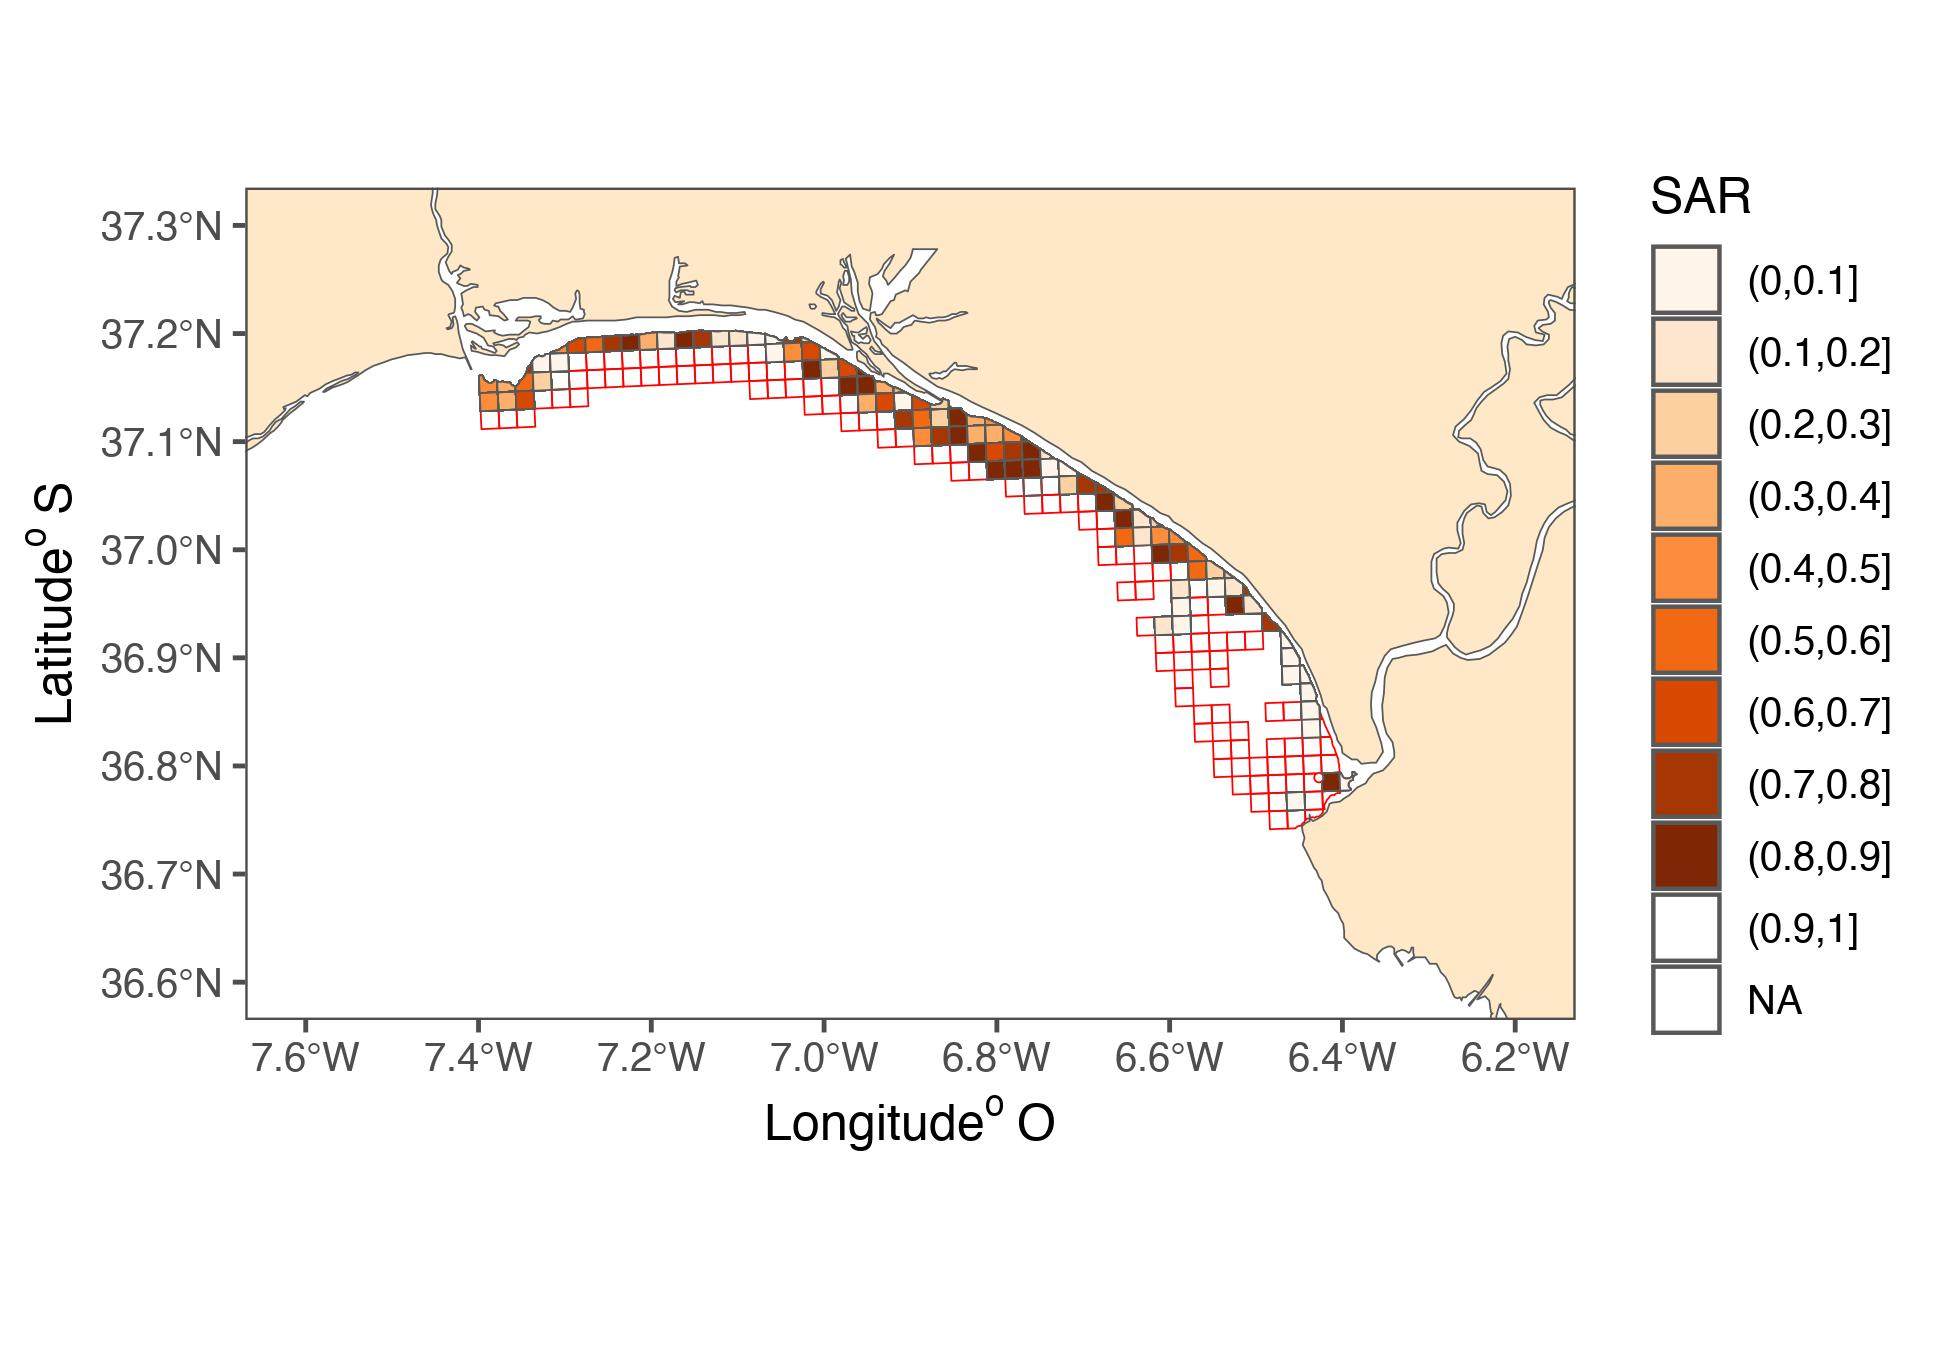
\includegraphics{SAR_Method_files/figure-latex/unnamed-chunk-17-1} \end{center}

Ahora trato de engrillar los habitat

Priebo el mapa

\begin{center}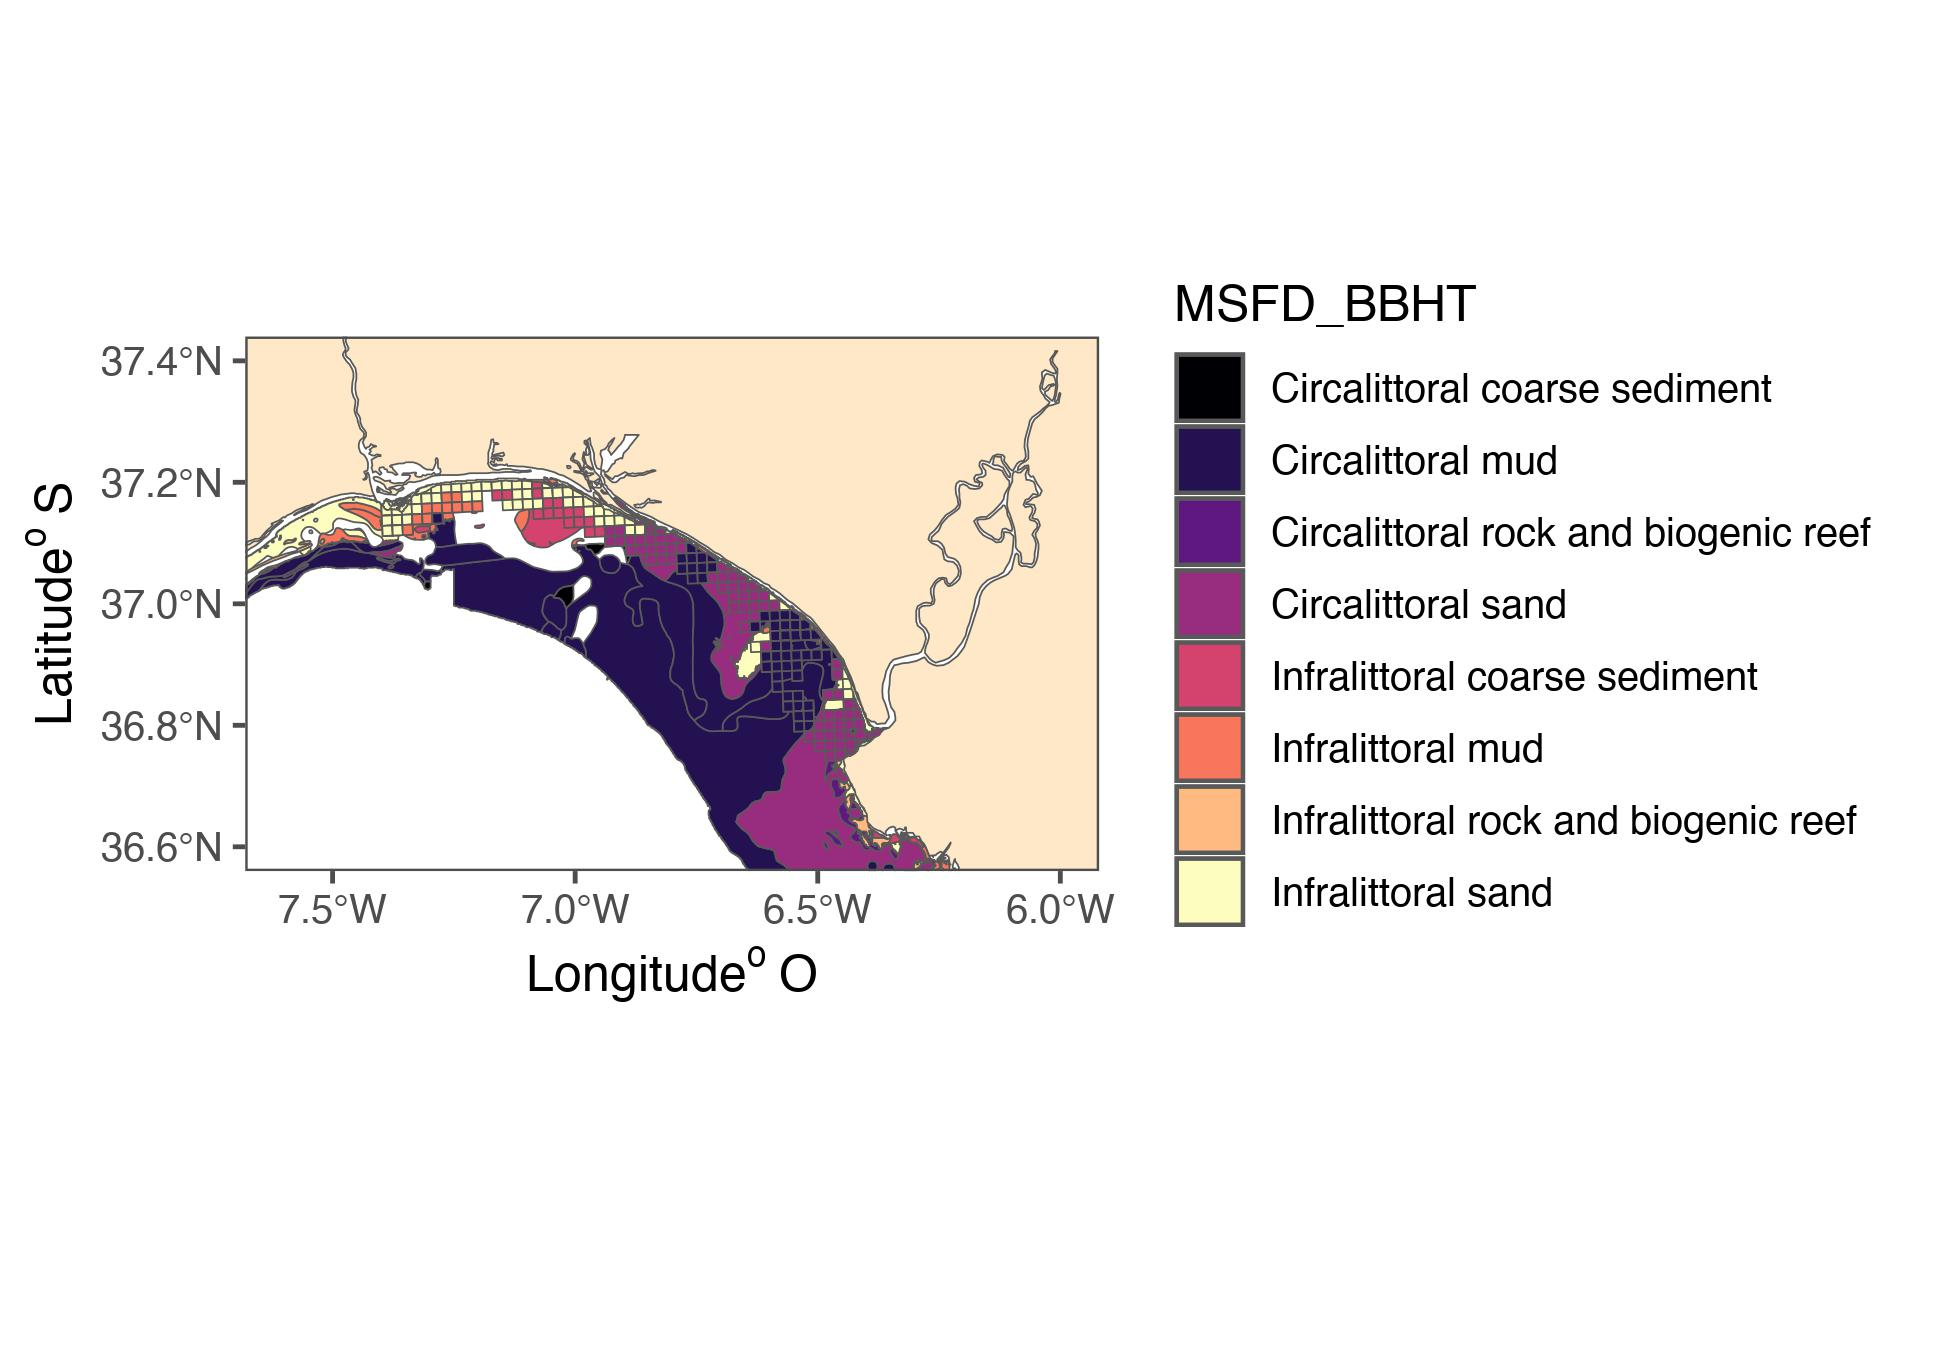
\includegraphics{SAR_Method_files/figure-latex/unnamed-chunk-19-1} \end{center}

Cuento cuantas estaciones hay por habitat.

\hypertarget{calculo-de-lances-por-estacion-o-por-habitat}{%
\subsection{Calculo de lances por estacion o por habitat}\label{calculo-de-lances-por-estacion-o-por-habitat}}

Pero para esto, primer debemos asignar un ID para cada operación.

\begin{verbatim}
## Simple feature collection with 6 features and 36 fields
## Geometry type: POLYGON
## Dimension:     XY
## Bounding box:  xmin: -6.471536 ymin: 36.89203 xmax: -6.449277 ymax: 36.92538
## Geodetic CRS:  WGS 84
## # A tibble: 6 x 37
## # Groups:   MATRICULA [1]
##   Estaciones     area FK_ERES FECHA        DIA HORA    FK_BUQUE MATRICULA PUERTO
##        <dbl>    <dbl>   <int> <date>     <int> <chr>      <int> <chr>     <chr> 
## 1        196 1305730.    1225 2008-09-04     4 09:15:~    22643 AL-2-1833 LEPE  
## 2        196 1305730.    1225 2008-09-04     4 09:18:~    22643 AL-2-1833 LEPE  
## 3        197 3098190.    1225 2008-09-04     4 09:21:~    22643 AL-2-1833 LEPE  
## 4        197 3098190.    1225 2008-09-04     4 09:27:~    22643 AL-2-1833 LEPE  
## 5        197 3098190.    1225 2008-09-04     4 09:27:~    22643 AL-2-1833 LEPE  
## 6        197 3098190.    1225 2008-09-04     4 09:30:~    22643 AL-2-1833 LEPE  
## # i 28 more variables: FK_TIPO_F <int>, F_LOCALIZA <chr>, N_X <dbl>, N_Y <dbl>,
## #   N_VELOCIDAD <dbl>, N_RUMBO <dbl>, N_SATELITES <int>, N_EN_PUERTO <int>,
## #   L_BACKUP <int>, FK_ACTIVI <int>, FK_ESTADO <int>, FK_MODAL <int>,
## #   ANO <dbl>, MES <dbl>, MANIOBRA <chr>, fecha_hora <dttm>, DISTANCIA <dbl>,
## #   diff <drtn>, diff_secs <dbl>, VELONUE <dbl>, DISTANCIA2 <dbl>, SA <dbl>,
## #   CELDAM2 <dbl>, length.out <int>, SAR <dbl>, geometry <POLYGON [°]>,
## #   diff_secs_next <dbl>, ID_Lance <int>
\end{verbatim}

Solo para visualizar, cambio el objeto a \texttt{data.frame}. Pero debo considerar \texttt{idlance4} para engrillar.

\hypertarget{discussion}{%
\section{DISCUSSION}\label{discussion}}

\hypertarget{conclusion}{%
\section{CONCLUSION}\label{conclusion}}

\newpage

\hypertarget{referencias}{%
\section*{REFERENCIAS}\label{referencias}}
\addcontentsline{toc}{section}{REFERENCIAS}

\hypertarget{refs}{}
\begin{CSLReferences}{1}{0}
\leavevmode\vadjust pre{\hypertarget{ref-Church2016}{}}%
Church, N. J., Carter, A. J., Tobin, D., Edwards, D., Eassom, A., Cameron, A., Johnson, G. E., Robson, L. M., \& Webb, K. E. (2016). {JNCC Pressure Mapping Methodology. Physical Damage (Reversible Change)-Penetration and/or disturbance of the substrate below the surface of the seabed, including abrasion}. \emph{JNCC Report No}, \emph{515}(December).

\leavevmode\vadjust pre{\hypertarget{ref-Cohan2012}{}}%
Cojan, M. (2012). \emph{{AN{Á}LISIS Y SEGUIMIENTO DE LA FLOTA DE DRAGAS HIDR{Á}ULICAS EN EL GOLFO DE C{Á}DIZ}} (pp. 1--23) {[}PhD thesis{]}.

\end{CSLReferences}

\end{document}
